%! Author = jonathan
%! Date = 5/27/25
\chapter{Evaluation}\label{ch:evaluation}
\begin{table}[h]
    \centering
    \caption{Implementation metrics of~\sysname using fully inlined NVSHMEM.}
    \label{tab:impl_metrics}
    \begin{tabular}{cc}
        \toprule
        \textbf{Metric} & \textbf{Value}\\ \hline
        Total lines of code (CUDA/C++) & 6820 \\
        Kernel stack frame size & 0 B \\
        Spill stores (per thread) & 0 \\
        Spill loads (per thread) & 0 \\
        Shared memory usage (per block) & 46 KB \\
        Registers per thread & 255 \\
        Max active blocks per SM & 2 \\
        Compilation time & 53 seconds \\
        Binary size & 29 MB\\
    \end{tabular}
\end{table}
We implement (Table~\ref{tab:impl_metrics}) and evaluate \sysname by addressing two main questions:
(1) Under what conditions does \sysname outperform state-of-the-art MoE systems,
and why (\S\ref{subsec:scalability-with-tokens-and-experts} -~\ref{sec:payload-efficiency})? and (2) How much GPU memory does
\sysname require for core data structures (\S\ref{sec:eval:memory})?
\section{Setup}\label{sec:setup}
We run experiments on a RunPod server with 8 $\times$ NVIDIA H100 80G GPUs, 125 GB of RAM, and 20 vCPUs.
We used PyTorch 2.6.0, CUDA 12.8, and Ubuntu 22.04.
All experiments use MoE transformer models configured with 16 attention heads,
an embedding dimension of 1024, and an FFN hidden size of 4096.
We use top-2 routing with a capacity factor of 1.0.
Note all baselines were evaluated using FP16 precision, while \sysname was evaluated on FP32 precision,
see \S\ref{ch:limitations-and-future-work} for more details.
We compare \sysname against several state-of-the-art MoE systems:
(1) \textbf{Comet}~\cite{comet},
(2) \textbf{FasterMoE}~\cite{fastermoe},
(3) \textbf{Megatron-LM}~\cite{megatron-lm}, and
(4) \textbf{DeepEP}~\cite{deepep}.
Comet and DeepEP rely on NVSHMEM for communication, while FasterMoE and Megatron-LM use NCCL.
We also evaluate \sysname on a multi-node environment and discuss our findings in \S\ref{sec:multi-node-evaluation}.
\section{Scalability with Tokens and Experts}\label{subsec:scalability-with-tokens-and-experts}
\begin{figure}[h!]
    \centering
    \subcaptionbox{Scaling with the number of tokens (E = 32).\label{fig:scalability-token}}{%
        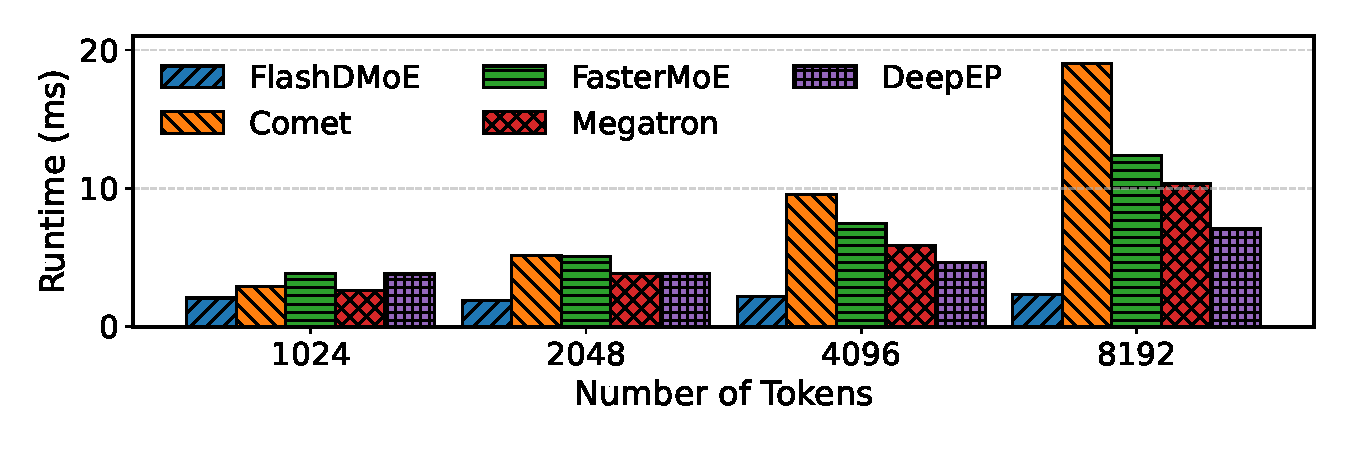
\includegraphics[width=\linewidth]{figures/scaling_tokens}
    }
    \subcaptionbox{Scaling with the number of experts (T = 8K)\label{fig:scalability-experts}}{%
        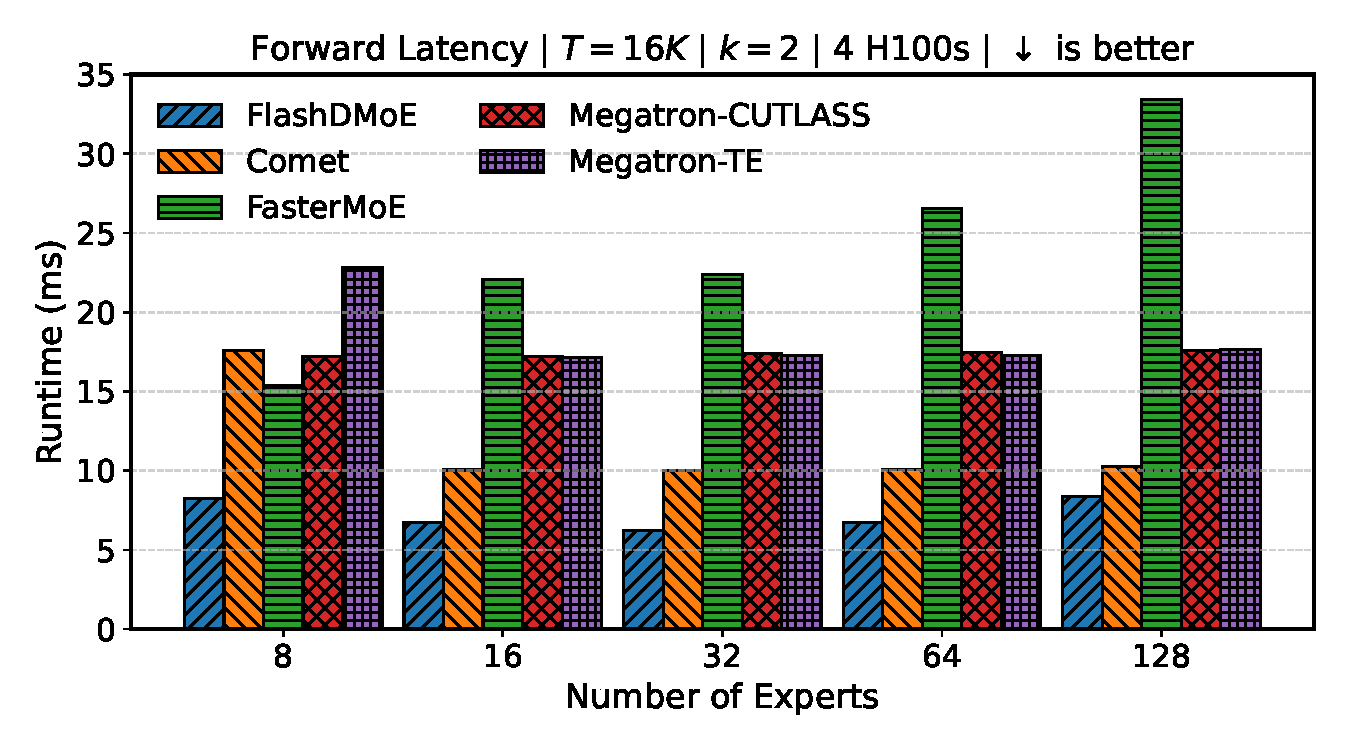
\includegraphics[width=\linewidth]{figures/scaling_experts}
    }
    \caption{Scalability with respect to the number of tokens and experts. All experiments use 8 GPUs.}
    \label{fig:scalability-token-experts}
\end{figure}
We first analyze the scalability of \sysname in two dimensions: the number of input tokens and the number of experts.
Figure~\ref{fig:scalability-token-experts} shows execution time for a single MoE layer on 8 GPUs.
\sysname outperforms baselines between \textbf{1.4X} to \textbf{9.5X} when scaling across sequence lengths and
between \textbf{1.2X} to \textbf{15X} across number of experts.
We provide raw performance numbers in \S\ref{sec:numerical-data}.

When scaling number of tokens (Fig.~\ref{fig:scalability-token}),
\sysname maintains near-constant execution time ($2.07-2.33$ ms).
In contrast, baselines incur significant runtime increases.
For example, Comet's runtime grows from 2.9 ms to 19 ms,
FasterMoE from 3.85 ms to 12.37 ms, Megatron-LM from 2.59 ms to 10.32 ms,
and DeepEP from 3.80 ms to 7.12 ms. \sysname avoids these overheads by overlapping computation and communication,
achieving stable performance despite higher token counts.
When scaling the number of experts (Figure~\ref{fig:scalability-experts}),
\sysname's runtime increases proportionally from 1.12 ms to 8.20 ms,
reflecting higher overhead from routing and processing additional experts.
Comet and Megatron-LM exhibit relatively flat runtimes (around 19 ms and 10.4 ms, respectively)
but at significantly higher latencies.
FasterMoE (7.9–22.65 ms) and DeepEP (6.03–11.3 ms)
show increasing runtimes due to overheads from inefficient communication or computation handling.
\section{GPU Scalability}\label{sec:gpu-scalability}
\begin{figure}[!ht]
    \centering
    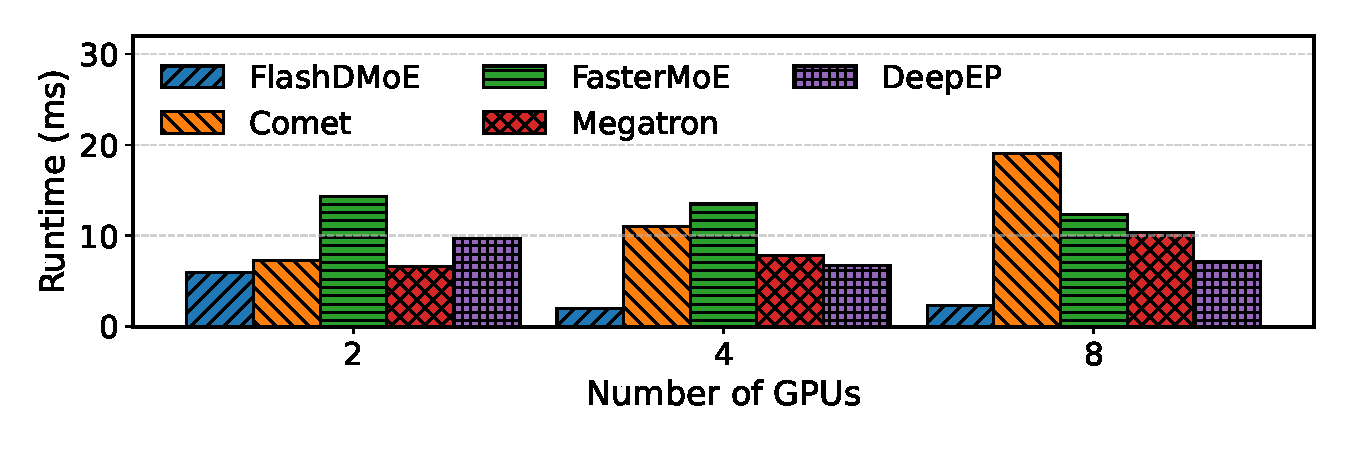
\includegraphics[width=\textwidth, keepaspectratio]{figures/scaling_gpus}
    \caption{Scalability with respect to the number of GPUs (E = 32, T = 8K).}
    \label{fig:scalability-gpus}
\end{figure}
Figure~\ref{fig:scalability-gpus} keeps tokens per GPU constant while scaling GPU count.
\sysname shows strong scalability, achieving a speedup from 5.99 ms (2 GPUs) to 1.98 ms (4 GPUs)
and maintaining performance at 8 GPUs (2.33 ms).
This highlights efficient inter-GPU communication and workload distribution.
Comet and Megatron-LM degrade notably (Comet: 7.26–19.01 ms; Megatron-LM: 6.59–10.32 ms),
indicating communication bottlenecks at scale.
FasterMoE shows modest improvements (14.28–12.37 ms),
and DeepEP displays a similar pattern to \sysname (9.65–7.12 ms) but with consistently higher runtimes.
\section{SM Utilization}\label{sec:sm-utilization}
\begin{figure}[!ht]
    \centering
    \subcaptionbox{Comparison of SM utilization, defined as the ratio of cycles in which SMs have at least one warp in flight to the total number of cycles~\cite{nsight-metrics}. Values represent the average SM utilization over 100 iterations. All experiments use T = 8K and E = 64 on two GPUs.\label{fig:sm-util}}{%
        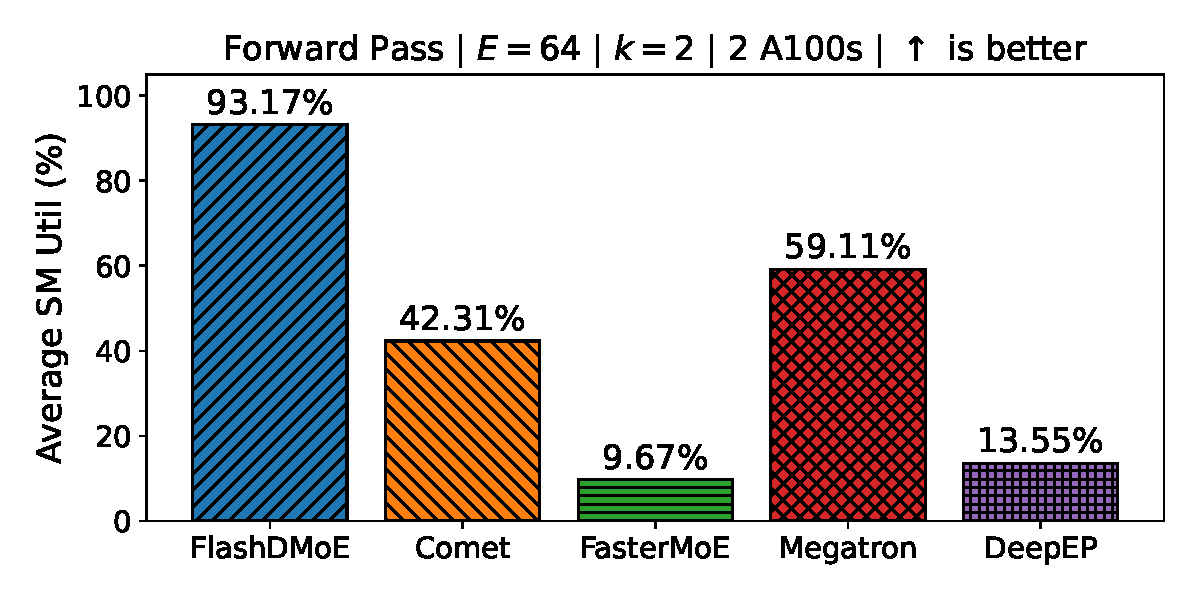
\includegraphics[width=0.7\linewidth]{figures/sm_util}
    }
    \hspace{2pt}
    \subcaptionbox{Payload efficiency. The y-axis shows the total number of bits transferred over NVLink with the same configuration. The x-axis shows the total layer execution time over 100 iterations. Both axes are log-scaled.
    % \byungsoo{Need to make sense of this result: why larger payload size for FasterMoE despite uniform configuration?}
    \label{fig:payload-efficiency}}{%
        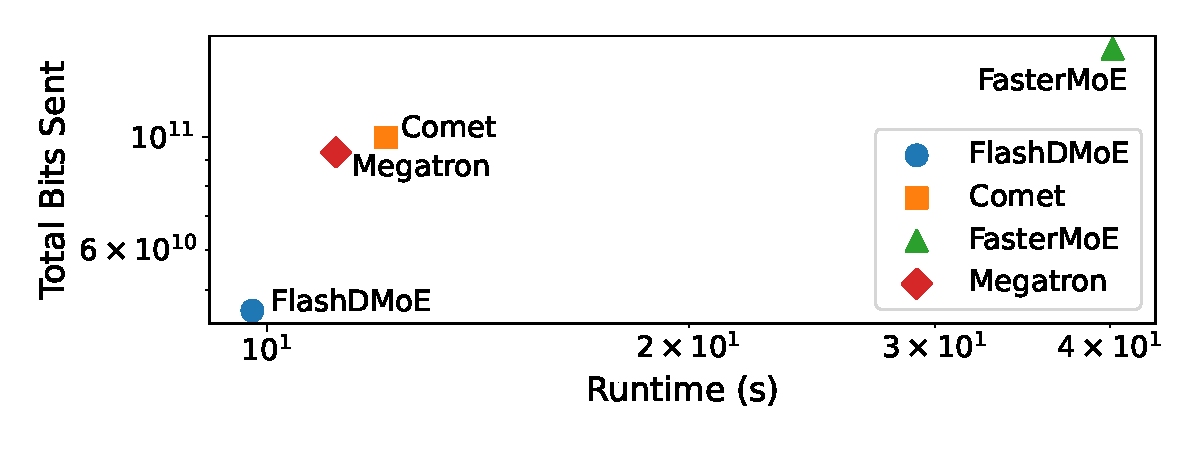
\includegraphics[width=0.7\linewidth]{figures/payload_efficiency}
    }
    \caption{Factors leading to performance improvement of \sysname.}
    \label{fig:sm-util-payload-efficiency}
\end{figure}
Figure~\ref{fig:sm-util} shows GPU utilization,
measured by the average SM utilization (fraction of GPU cycles with active warps~\cite{nsight-metrics}).
\sysname achieves over 90\% SM utilization, showing effective fine-grained task scheduling and reduced idle GPU time.
\section{Payload Efficiency}\label{sec:payload-efficiency}
We next evaluate payload efficiency (Figure~\ref{fig:payload-efficiency})
by measuring the volume of data transferred over NVLink.
Traditional MoE frameworks communicate zero-padded tokens,
inflating network payloads.
In contrast, \sysname's in-place padding approach transmits only active tokens,
reducing communication volume substantially and resulting in better runtime performance.
\section{Multi-Node Evaluation}\label{sec:multi-node-evaluation}
\subsection{Setup}\label{subsec:setup}
In this experiment, we seek to evaluate \sysname in the multi-node setting.
We use 4 nodes, where each node comprises 4 A100 GPUs fully interconnected via NVLink.
Across nodes, each GPU uses a single NIC providing 25 GB/s of bandwidth.
We set the number of experts to be $16$ and assign each GPU to host only one,
so the number of local experts is $1$.
Note that we define MIV formally as follows:
\[
    MIV = \frac{Tokens}{Experts} * local\_{experts} * precision * hidden\_size * 2 * n_{rg}
\]
where $n_{rg}$ is the number of remote peers and the multiplicative
factor of $2$ accounts for communication rounds (dispatch and combine).
$n_{rg} = 12$ for this experiment.
\subsection{Results}\label{subsec:results}
\begin{figure} [!ht]
    \centering
    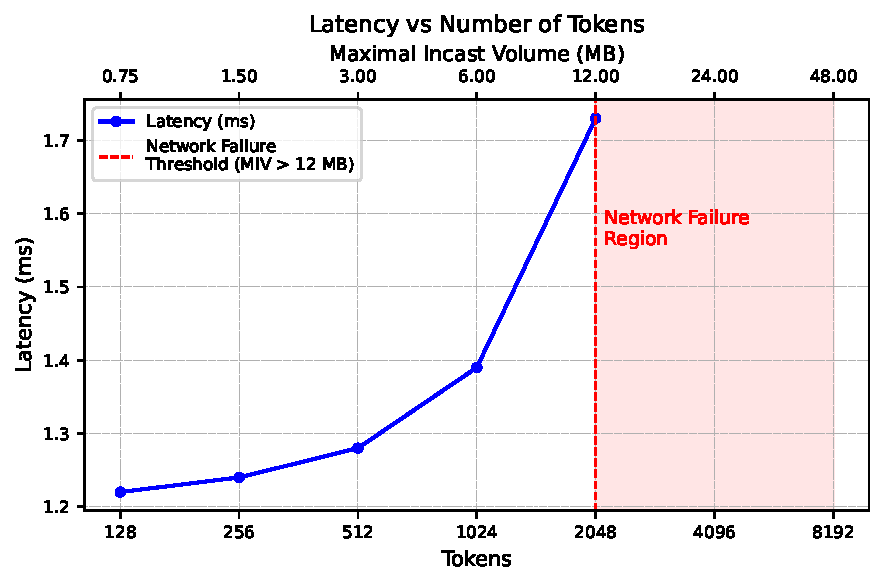
\includegraphics[width=4in,keepaspectratio]{figures/multi_node_fail}
    \caption{Multi-node Latency evaluation.
    Embbeding dimension is $1024$ and FFN intermediate size is $4096$.
    We define Maximal Incast Volume (MIV) as the worst case upper bound for data volume that a
    NIC receives in a single incast occurence.}
    \label{fig:multi_fail}
\end{figure}
We observe a sublinear increase in latency as we scale the number of tokens.
However, we observe at $Tokens > 2048$, that the application fails to terminate
due to failure to receive expectant messages.
We hypothesize this failure to be due to buffer overflow at the networking hardware layer as is common for applications
that generate many and large messages~\cite{nerscNetworkNERSC} like our system.
We note that this failure is addressable by tuning hardware configurations~\cite{ofiwgFi_cxi7} but we consider
this exploration as an exercise orthogonal to this work.
\section{Memory Overhead}\label{sec:eval:memory}
We measure the GPU memory required for the symmetric tensor $L$ and runtime bookkeeping state of \sysname.
Memory overhead depends primarily on the tile size, expert capacity (EC), and the number of experts ($E$).
Table~\ref{tab:memory-overhead} summarizes memory overhead under various configurations,
confirming that \sysname maintains a modest and predictable memory footprint.
\begin{table}[!ht]
    \centering
    \caption{Memory overhead (tile size $bM = 128$, $Size(T) = \text{Tokens} * 4KB$).}
    \label{tab:memory-overhead}
    \setlength{\tabcolsep}{2pt}
    \renewcommand{\arraystretch}{0.9}
    \begin{tabular}{ccccccc}
        \toprule
        \textbf{Tokens} & \textbf{Experts} & \textbf{EC} & \textbf{max(bM, EC)} & \textbf{Bookkeeping (MB)} & $Size(L)$ \textbf{(MB)} & \textbf{Total (MB)} \\
        \midrule
        4K  & 16  & 256  & 256  & 64.57  & 64.00  & 128.57 \\
        4K  & 32  & 128  & 128  & 64.55  & 64.00  & 128.55 \\
        4K  & 64  & 64   & 128  & 128.90 & 128.01 & 256.91 \\
        4K  & 128 & 32   & 128  & 257.96 & 256.02 & 513.98 \\
        \midrule
        8K  & 16  & 512  & 512  & 128.95 & 128.01 & 256.95 \\
        8K  & 32  & 256  & 256  & 128.90 & 128.01 & 256.91 \\
        8K  & 64  & 128  & 128  & 128.90 & 128.01 & 256.91 \\
        8K  & 128 & 64   & 128  & 258.15 & 256.02 & 514.17 \\
        \midrule
        16K & 16  & 1024 & 1024 & 257.89 & 256.02 & 513.90 \\
        16K & 32  & 512  & 512  & 257.79 & 256.02 & 513.81 \\
        16K & 64  & 256  & 256  & 257.80 & 256.02 & 513.81 \\
        16K & 128 & 128  & 128  & 258.53 & 256.02 & 514.54 \\
        \bottomrule
    \end{tabular}
\end{table}
\clearpage
\section{Numerical Data}\label{sec:numerical-data}
\begin{table}[!ht]
    \centering
    \caption{Latency (ms) comparison across different numbers of tokens (Figure~\ref{fig:scalability-token}).}
    \label{tab:latency-tokens}
    \setlength{\tabcolsep}{5pt}
    \renewcommand{\arraystretch}{0.9}
    \begin{tabular}{cccccc}
        \toprule
        \textbf{Tokens} & \textbf{FlashDMoE} & \textbf{Comet} & \textbf{FasterMoE} & \textbf{Megatron} & \textbf{DeepEP} \\
        \midrule
        1024  & 2.07 & 2.87 & 3.85 & 2.59 & 3.80 \\
        2048  & 1.90 & 5.12 & 5.04 & 3.83 & 3.83 \\
        4096  & 2.19 & 9.54 & 7.44 & 5.83 & 4.62 \\
        8192  & 2.33 & 19.01 & 12.37 & 10.32 & 7.12 \\
        \bottomrule
    \end{tabular}
    \vspace{-0.4cm}
\end{table}
\begin{table}[!ht]
    \centering
    \caption{Latency (ms) comparison across different numbers of experts (Figure~\ref{fig:scalability-experts}).}
    \label{tab:latency-experts}
    \setlength{\tabcolsep}{5pt}
    \renewcommand{\arraystretch}{0.9}
    \begin{tabular}{cccccc}
        \toprule
        \textbf{Experts} & \textbf{FlashDMoE} & \textbf{Comet} & \textbf{FasterMoE} & \textbf{Megatron} & \textbf{DeepEP} \\
        \midrule
        16  & 1.20 & 19.01 & 11.38 & 10.47 & 5.59 \\
        32  & 2.33 & 19.01 & 12.37 & 10.32 & 7.12 \\
        64  & 4.20 & 19.21 & 16.64 & 10.47 & 7.49 \\
        128 & 8.20 & 19.36 & 22.65 & 10.47 & 11.30 \\
        \bottomrule
    \end{tabular}
    \vspace{-0.4cm}
\end{table}
\begin{table}[!ht]
    \centering
    \caption{Latency (ms) comparison across different numbers of GPUs (Figure~\ref{fig:scalability-gpus}).}
    \label{tab:latency-gpus}
    \setlength{\tabcolsep}{5pt}
    \renewcommand{\arraystretch}{0.9}
    \begin{tabular}{cccccc}
        \toprule
        \textbf{GPUs} & \textbf{FlashDMoE} & \textbf{Comet} & \textbf{FasterMoE} & \textbf{Megatron} & \textbf{DeepEP} \\
        \midrule
        2 & 6.00 & 7.26 & 14.28 & 6.59 & 9.65 \\
        4 & 1.98 & 10.98 & 13.59 & 7.82 & 6.72 \\
        8 & 2.33 & 19.01 & 12.37 & 10.32 & 7.12 \\
        \bottomrule
    \end{tabular}
    \vspace{-0.4cm}
\end{table}